% LINGI2255 - Software Development Project
% Final report
\documentclass[11pt, a4paper]{article}   	% use "amsart" instead of "article" for AMSLaTeX format
\usepackage[T1]{fontenc}
\usepackage[utf8]{inputenc}
\usepackage{lmodern}
\usepackage[UKenglish]{babel}
\usepackage{graphicx}

\usepackage{amssymb}
\usepackage{xcolor}
\usepackage{hyperref}
\usepackage{url}
\usepackage{csquotes}
\usepackage{enumitem}
\usepackage{lipsum}
\usepackage{listings}
\usepackage{textcomp}
\lstset{language=Python}

\newcommand{\tbf}[1]{\textbf{#1}}
\newcommand{\tit}[1]{\textit{#1}}
\newcommand{\ttt}[1]{\texttt{#1}}
\newcommand{\noi}{\noindent}
\newcommand{\shellcmd}[1]{\\\indent\indent\texttt{\footnotesize\$ #1}\\}
\newcommand{\vshellcmd}[1]{\\\indent\indent\texttt{\footnotesize(venv)\$ #1}\\}
\newcommand{\pcmd}[1]{\\\indent\indent\texttt{\footnotesize> > > #1}\\}

\hypersetup{
    bookmarks=true,         % show bookmarks bar?
    unicode=false,          % non-Latin characters in Acrobat’s bookmarks
    pdftoolbar=true,        % show Acrobat’s toolbar?
    pdfmenubar=true,        % show Acrobat’s menu?
    pdffitwindow=false,     % window fit to page when opened
    pdfstartview={FitH},    % fits the width of the page to the window
    pdftitle={My title},    % title
    pdfauthor={Author},     % author
    pdfsubject={Subject},   % subject of the document
    pdfcreator={Creator},   % creator of the document
    pdfproducer={Producer}, % producer of the document
    pdfkeywords={keyword1} {key2} {key3}, % list of keywords
    pdfnewwindow=true,      % links in new PDF window
    colorlinks=true,       % false: boxed links; true: colored links
%    linkcolor=red,          % color of internal links (change box color with linkbordercolor)
    citecolor=green,        % color of links to bibliography
    filecolor=magenta,      % color of file links
    urlcolor=blue           % color of external links
}

\lstset{%
    inputencoding=utf8,
        extendedchars=true,
        literate=%
        {é}{{\'{e}}}1
        {è}{{\`{e}}}1
        {ê}{{\^{e}}}1
        {ë}{{\¨{e}}}1
        {û}{{\^{u}}}1
        {ù}{{\`{u}}}1
        {â}{{\^{a}}}1
        {à}{{\`{a}}}1
        {î}{{\^{i}}}1
        {ô}{{\^{o}}}1
        {ç}{{\c{c}}}1
        {Ç}{{\c{C}}}1
        {É}{{\'{E}}}1
        {Ê}{{\^{E}}}1
        {À}{{\`{A}}}1
        {Â}{{\^{A}}}1
        {Î}{{\^{I}}}1
}

\title{Brief Article}
\author{The Author}
%\date{}							% Activate to display a given date or no date

\begin{document}
%\maketitle

%%%%%% Section
\section{Introduction}

%%%%%% Section
\section{Overall project impressions}

As we approach the end of this project, we take a look back at our previous reports and try to analyze what we did right and what we did wrong. What we were able to implement the way we intended and what we had to change in order to complete this project in time. This analysis should help us in our future projects and tell us whether we were too ambitious or if we could have done much more.

\subsection{The development plan}

We will start by taking a look at the development plan since it is fairly easy to notice whether we were able to respect it or not. Even though the development plan we put in place helped us visualize the amount of work to be done and how we could manage our time, we ran into some difficulties when it came to actually respect this plan.

Indeed, this development plan was done without much knowledge of how Django works and thus neglected some important parts of the implementation. For instance, the overall design of the website was not considered in the development plan whereas in reality it took us some time to find a way to make our application look as appealing as possible. 
This plan didn't take into consideration the fact that some group had no experience with the framework at all, which made some tasks drag on for more time that what was initially excpected since we had to familiarize ourselves with the framework before being able to program anything. 

\subsection{Absent modules}
Thankfully, we foresaw that we would most likely run into some problems, which is why we decided that some modules would be optionnal. These modules could be implemented if we had enough time but would be the first ones to be dropped if we had difficulties completing the project in due time. These modules were mostly secondary and the application would still be viable without them.

Because of the difficulties mentionned above, we had to drop some of these modules. We can thus notice that the "events" module, the "calendar" module, the "personal network" module and the "notifications" were not fully implemented. Some of the aforementioned modules are still present to some extent but were not implemented in the way the client would have wanted them to be implemented. We notice that some of these modules were not marked as optional in our development plan, but it is our belief that even without them, the application is still functional and could be used in real life settings. 

Even after dropping these modules, we still had little time left to implement our extension and simulation after the kernel was done. However, we believe we did a good job at implenting those and that they add a real value to our application.

\subsection{Additional modules}
While we can see that we had some trouble completing some features of the application, we can also notice that we actually had some ideas during the implementation phase for some functionnalities which we hadn't discussed in previous reports. For instance, we noticed that a member could join any branch and that there was no way, even for an administrator, to stop a member from joining a branch. We thus decided to add a "ban" functionnality, giving administrators the opportunity to stop someone from joining a branch. We hope this functionnality won't be needed in the end, but, as the saying goes, better safe than sorry. We also added the possibility the increase the font size to help people with vision difficulties to read the application's content more easily.  We also integrated Google Maps in our application to facilitate the visualization of the distance to be travelled in order for someone to help someone else. Even though none of these functionnalities were mentioned in our previous reports, it is our belief that they make our application a better and easier to use one.\\

It could be argued that it would have been better to start by finishing what was asked before adding features which were not asked. We have a quite simple answer to this : we did not realize we would have to drop these functionnalities at the time we implemented the ones which weren't required. In the end, we realize we were too ambitious in our previous reports and at the start of the implementation phase and it cost us some functionnalities. We also realize that we had to change our vision of the system as time went on because our vision did not always match the way Django worked. The next section will present all the functionnalities we did implement and will hopefully show why we still think we met most of our goals regarding the functional and non-functional requirements set at the start of this project.

%%%%%% Section
\section{Product}

\subsection{Features}

\subsubsection{Sign in}

When you have not sing up, you can only access the home page(you can see some jobs but you can't see details) and the news, help, about, what's care4care and jobs@care4care sections.
\newline

On the top of the page you can modify the language, log in and sign up. When you click on sign up, you reach a form where basic informations are required and if you want to be a member or a non-member. After completing this one, you can confirm your inscription and then a mail for validate your account his send to your mail address.
\newline

You can sign in whit your social account, this will auto complete your information.

\subsubsection{Profile}

You can sign in with the button which has the same name on the top of the page. At that time you will see a more complete menu on the right and new features on the top. You can for example search a job or a other member you get a specific mail box for your account care4care but this will be explain later.
\newline

For access your profile you have to click on this button 
\includegraphics[width=0.4cm]{user_icon.png} and click on my profile in the drop down menu or in the left menu in my profile section, then you get a new page where you can see all information about you. I will list you all possible actions possible from this page:
\begin{enumerate}
  \item \textbf{Modify your profile :} You can click on "
\includegraphics[width=0.4cm]{edit_icon.png}Edit" next to the username. There you can update all your personal informations (there are more informations than in the inscription page but you are not forced to complete everything once).
  \item \textbf{Social network :} You can link your account with your social network, even all if desired. You can edit them thereafter if needed (example: delete it).
  \item \textbf{Emergency contact :} "
\includegraphics[width=0.2cm]{plus_icon.png} Add" This allow you to fill information about a close friend or a family member to contact in emergency case. More than one contact are allowed.  
\end{enumerate}
In the top of the main profile page, a menu is available, here are the actions and their usage:
\begin{enumerate}
  \item \textbf{Profile :} The default page all informations about this page have been described just on the section above.
  \item \textbf{Favorites :} There you can add other member to your favorites network. Your favorites member can see specific offer and demand from you.
  \item \textbf{My network :} This your personal network. That help for other member which want to see your personal information. you could for example add your doctor there.
  \item \textbf{Ignored users :} If a member is annoying you, you can add him to your ignored list. It will hide all his demands and offers (except for superuser and branch officer)
  \item \textbf{Statistiques :} See section \ref{sec:section_personal_stats}
\end{enumerate}

\subsubsection{Credit}

Credit page are available in left menu in "my profile" section. On this page you can see your credit, some small statistics, jobs historic, jobs pending. You can perform gift to other member or administration (with a love message).

\subsubsection{Verified Member}

\paragraph{Make a demand}
For become a verified member, you have to click on this button 
\includegraphics[width=0.4cm]{user_icon.png} and click on "Become verified" in the drop down menu or you can use the left menu in the profile section.
You have to complete all missing informations about you. After validation there is a second page asking you two recommendation letters and your criminal record.

\paragraph{Manage a demand for branch officer or superuser}
When a member make a demand you can see it in the branch page where the member belong(for the branch page, use the left menu branch section). There is a list with all verified demand. When you click on a demand you can see all informations about the member and visualize his documents. At this point you have tree choices. 
\begin{itemize}
	\item Fix an appointment.
	\item Grant the status (a success message is automatically send to the member
	\item refuse the status (a refuse message is automatically send to the member
\end{itemize}

\subsubsection{Search}

\paragraph{Search a member}
You can search for an other member in the search bar on the top menu. It will return all members witch contain the string entered in their username, first name, last name.

\paragraph{Search a job}
Using the left menu click on search for a job. At this point you can specify 
\begin{enumerate}
	\item If you want see offers, demands or both.
	\item Category
	\item Who can see the demands or offers (All, favorites members, verified members)
	\item Time slot
\end{enumerate}
If you don't pick anything in a list, the system will consider that you want all items in the list.
Click on continue to start the search and you will see all available and not closed job.

\subsubsection{Branch}

\paragraph{Join a branch}
Everybody(except superuser witch is in all branch) can join a branch in the left menu to the section branch $\to$ "Join branch".

\paragraph{Create a branch}
Superuser and verified member can create a branch using the left menu to the section banch -> "create a new branch". You have to specify a name for the branch and a location.

\paragraph{Branch detail}
To access the details on a specific branch, left menu to the section branch -> name of the branch.
\begin{enumerate}
	\item \textbf{For member and verified member :} You can "ask for help" or "offer your help" in the branch with the specific button. All the offers and demands in the branch that you are allowed to see are visible in the branch page.
You can see details on click.
On the top right of the page you can leave the branch.
	\item \textbf{For branch officer and superuser :} You see everything that member and verified member can see. Moreover, branch statistics are available and you can manage branch's offers and demands. You can remove and ban a user from the branch (a ban list is available for unban).
	\item \textbf{For branch creator :} same as superuser but you can remove the branch with all his demands and offers.
\end{enumerate}

\subsubsection{Mailbox}

Every member get a mailbox after sign in, he can use it for sending mail to other member or administrator. Sometimes the system use the mailbox automatically in order to reduce the administrator workload.

\input{statistics.texpart}

%%%%%% Section
\section{Technical discussion}

\subsection{Virtual Environment}

We use \texttt{pyvenv}, a tool that can create virtual environment in \texttt{Python}, to keep the dependencies required by our project in a single place. It creates a folder which contains all the necessary executables to use the packages that our project will need. To create the virtual environment :
\shellcmd{pyvenv venv}
To activate the environment :
\shellcmd{source venv/bin/activate}
Once your virtual environment installed and activated, you can install the dependencies of \texttt{Care4Care}. All the dependencies are listed in the file requirements.txt. You can install all of them with the following command:
\vshellcmd{pip install -r requirements.txt}

\subsection{Create the database}
Once you're in a proper virtual environment with all dependencies installed, you can create the database. To do so, you can go in the root of our \texttt{Django} project and use the built-in command :
\vshellcmd{./manager.py syncdb}
At the end, you will ask to create a ``super user'', you can create a user ``care4care''. If you want to populate the database with some demo datas, you can run :
\vshellcmd{./manager.py loaddata data\_demo.json}

\subsection{Run the project}
One you're in the virtual environment with all dependencies installed and the dabatase created, you can launch the development server :
\vshellcmd{./manager.py runserver}
When the server is launched, you can surf the website in your browser at \url{http://localhost:8000}. 

\subsection{File hierarchy}
The project is divised in three ``Django applications'' wich are differents folders in our project :
\begin{description}[noitemsep]
\item[- main] contains everything about users management
\item[- branch] contains everything about branch and jobs (demands and offers)
\item[- news] contains everything about the news system
\end{description}

Each of these ``Django applications'' contains typic files/folders :
\begin{description}[noitemsep]
\item[- migrations/] is a folder containing migrations files. This is the Django’s way of propagating changes we make in our models (adding a field, deleting a model, etc.) into our database schema.
\item[- templates/] is a folder containing our templates. A template is simply a text file (ofter HTML). It contains variables, which get replaced with values when the template is evaluated, and tags, which control the logic of the template.
\item[- Templatestags/] is a folder in wich we will extend the template engine by defining custom tags, and then make them available in our templates.
\item[- static/] is a folder in wich we will put every static files (images, javascript, photos, etc.) used by the application.
\item[- \_\_init\_\_.py] used to mark the folder on disk as Python package directory.
\item[- admin.py] contains all the logic for the auto-generated django-admin.
\item[- forms.py] contains all the forms used by the ``Django application'' and the validation logic.
\item[- models.py] contains all the models used by the ``Django application''. Models are the source of information about data. Each attribute of a model represents a database field. 
\item[- tests.py] contains unit tests.
\item[- urls.py] contains every URLs available for the ``Django application''.
\item[- views.py] contains the logic of every views (linked to an URL) for the ``Django application''.
\end{description}

There is some more specific folders in the root of our project that need to be describe :
\begin{description}[noitemsep]
\item[- care4care/] contains the settings.py file where you can define all settings relative to our project.
\item[- templates/] contains templates that are linked to a third-party application.
\item[- static/] contains all static files not related to a specific application but more about the whole project.
\item[- media\_root/] contains every files uploaded by users via the website.
\item[- locale/] contains translations (i18n) of the project.
\end{description}

And there is some more specific files in the root of our project that need to be describe :
\begin{description}[noitemsep]

\item[- make\_locale.sh] generates translations .po files into ``locale/''. These files contains every sentences to be translated.
\item[- compile\_locale.sh] compiles translations .po files into usable translations .mo files.
\item[- manage.py] is generated by Django. This is the command-line utility for administrative tasks. 
\item[- start.sh] will run the project in a gunicorn server for production environment.
\end{description}

\subsection{Django : How does it works ? A simple example}

To understand how Django works, we'll use as an example the page that allows an user to add an emergency contact. Everything shown here is present in our code in the application ``main''.

\subsubsection{Models}
First, we have to create a model (wich is represnted by a Class) in \texttt{models.py}:

\begin{lstlisting}[language=Python, basicstyle=\footnotesize]
PRIORITY = (
    (1, _("A contacter en premier")), # To contact first
    (2, _("A contacter")), # To contact 
    (3, _("A contacter en dernier")) # To contact ultimately
    )

class EmergencyContact(CommonInfo):
    user = models.ForeignKey('User', related_name="emergency_contacts")
    order = models.IntegerField(default=0, \
      verbose_name=_("Ordre de priorité"), choices=PRIORITY)

    class Meta:
        ordering = ['order']
\end{lstlisting}

Class EmergencyContact inherits from class CommonInfo. CommonInfo contains fields : first\_name, last\_name, location, latitude, longitude, phone\_number, mobile\_number and languages. So EmergencyContact already got all these attributes. Plus, we add two other : user and order. User is a ForeignKey to the class User. It will be useful to know wich User is associated with an emergency contact. And the order field is useful to know wich emergency contact you should contact first.


This class will create all necessary entries in the databases. It also gives us an easy API to make request to the database. So, if we want to get all the EmergencyContact of user id number 4, we can write:
\pcmd{EmergencyContact.objects.filter(user\_\_id=4).all()}

In the Meta class, we wrote ``ordering = ['order']'', this has the effect of sorting the results of our requests per the field ``order''.

\subsubsection{View}
The view is the logic of the page.

\begin{lstlisting}[language=Python, basicstyle=\footnotesize]
# in forms.py
class EmergencyContactCreateForm(forms.ModelForm):
    class Meta:
        model = EmergencyContact
        exclude = ['user', 'latitude', 'longitude']

# in views.py
class AddEmergencyContact(CreateView):
    """A view for add an emergency_contact"""
    template_name = 'profile/emergency_contact.html'
    form_class = EmergencyContactCreateForm
    model = EmergencyContact

    @method_decorator(login_required)
    def dispatch(self, *args, **kwargs):
        obj = self.get_object()
        if obj.id != self.request.user.id and not self.request.user.is_superuser:
            return redirect(obj.get_absolute_url())
        return super(AddEmergencyContact, self).dispatch(*args, **kwargs)

    def get_object(self, queryset=None):
        return User.objects.get(pk=self.kwargs['user_id'])

    def form_valid(self, form):
        form.instance.user = User.objects.get(pk=self.kwargs['user_id'])
        return super(AddEmergencyContact, self).form_valid(form)

    def get_success_url(self):
        return self.get_object().get_absolute_url()
\end{lstlisting}

We will use a Generic View (CreateView) to create a new Emergency Contact. Since the administrator (superuser) can be able to add an emergency contact to any user, we will have to specify for wich user we create an emergency contact. To do so, we will give the user id in the url linked to this view (see next section). We can get the number id via ``self.kwargs['user\_id']''. Since this will be useful, we define a method \texttt{get\_object} that will get the user object in database. Then, we will override the dispatch method. In this method, we will first add the method decorator \texttt{login\_required}. This decorator will assure that the user is connected. If not, it will brings the user to the login page. In the method, we will check that the user have got enough right to create an emergency contact for the user (self.get\_object). 

We specify the form via the field form\_class. So we created a class EmergencyContactCreateForm. This form is an ModelForm, so it will be automatically generated from the model EmergencyContact as we can read in his Meta class. We can see that we exclude three fields that we don't want here : user, latitude and longitude. So we will ask the user all fields of the model class EmergencyContact except these three.

We override the method form\_valid to link the current user (self.get\_object) with the emergency contact in creation.

At least, we override the method \texttt{get\_success\_url}. When the form is valid, the user will be redirect the profile of the user. If the form is not valid, the CreateView logic will point out the error to the user and ask him to correct it.

\subsubsection{URLs}

In the file \texttt{urls\_profile.py} (extension of \texttt{urls.py}), we will add the following entry in the urlpatterns :

\begin{lstlisting}[language=Python, basicstyle=\footnotesize]
  url(r'^profile/add_emergency_contact/(?P<user_id>\d+)/',
      AddEmergencyContact.as_view(),
      name='add_emergency_contact'), 
\end{lstlisting}

We can find the famous ``user\_id'' that will be use in the method \texttt{get\_object} in our view. Also, we give a name to our url. This is usefull to not remember the used url since we will be able to write the url in a template with the templatetag url : ``\{\% url 'add\_emergency\_contact' request.user.id \%\}''.

\subsubsection{Template}

The final step is to write the template specified in our view : \texttt{'profile/emergency\_contact.html'}:

\begin{lstlisting}[language=HTML, basicstyle=\footnotesize]





[..]
    <form action="." role="form" method="post">
      
       [..]
          
        [..]
        <button type="submit" class="btn btn-success btn-lg btn-block">
             &nbsp; </button>
        [..]
    </form>
[..]

\end{lstlisting}

We can see that render our form is easy as ``\{\% bootstrap\_form form \%\}''. We just need the <form> and a submit button. The rest is for the style of the page.

And that's all, we have created a page with the possibility of creating an emergency contact linked to a user :

\begin{figure}[!ht]
   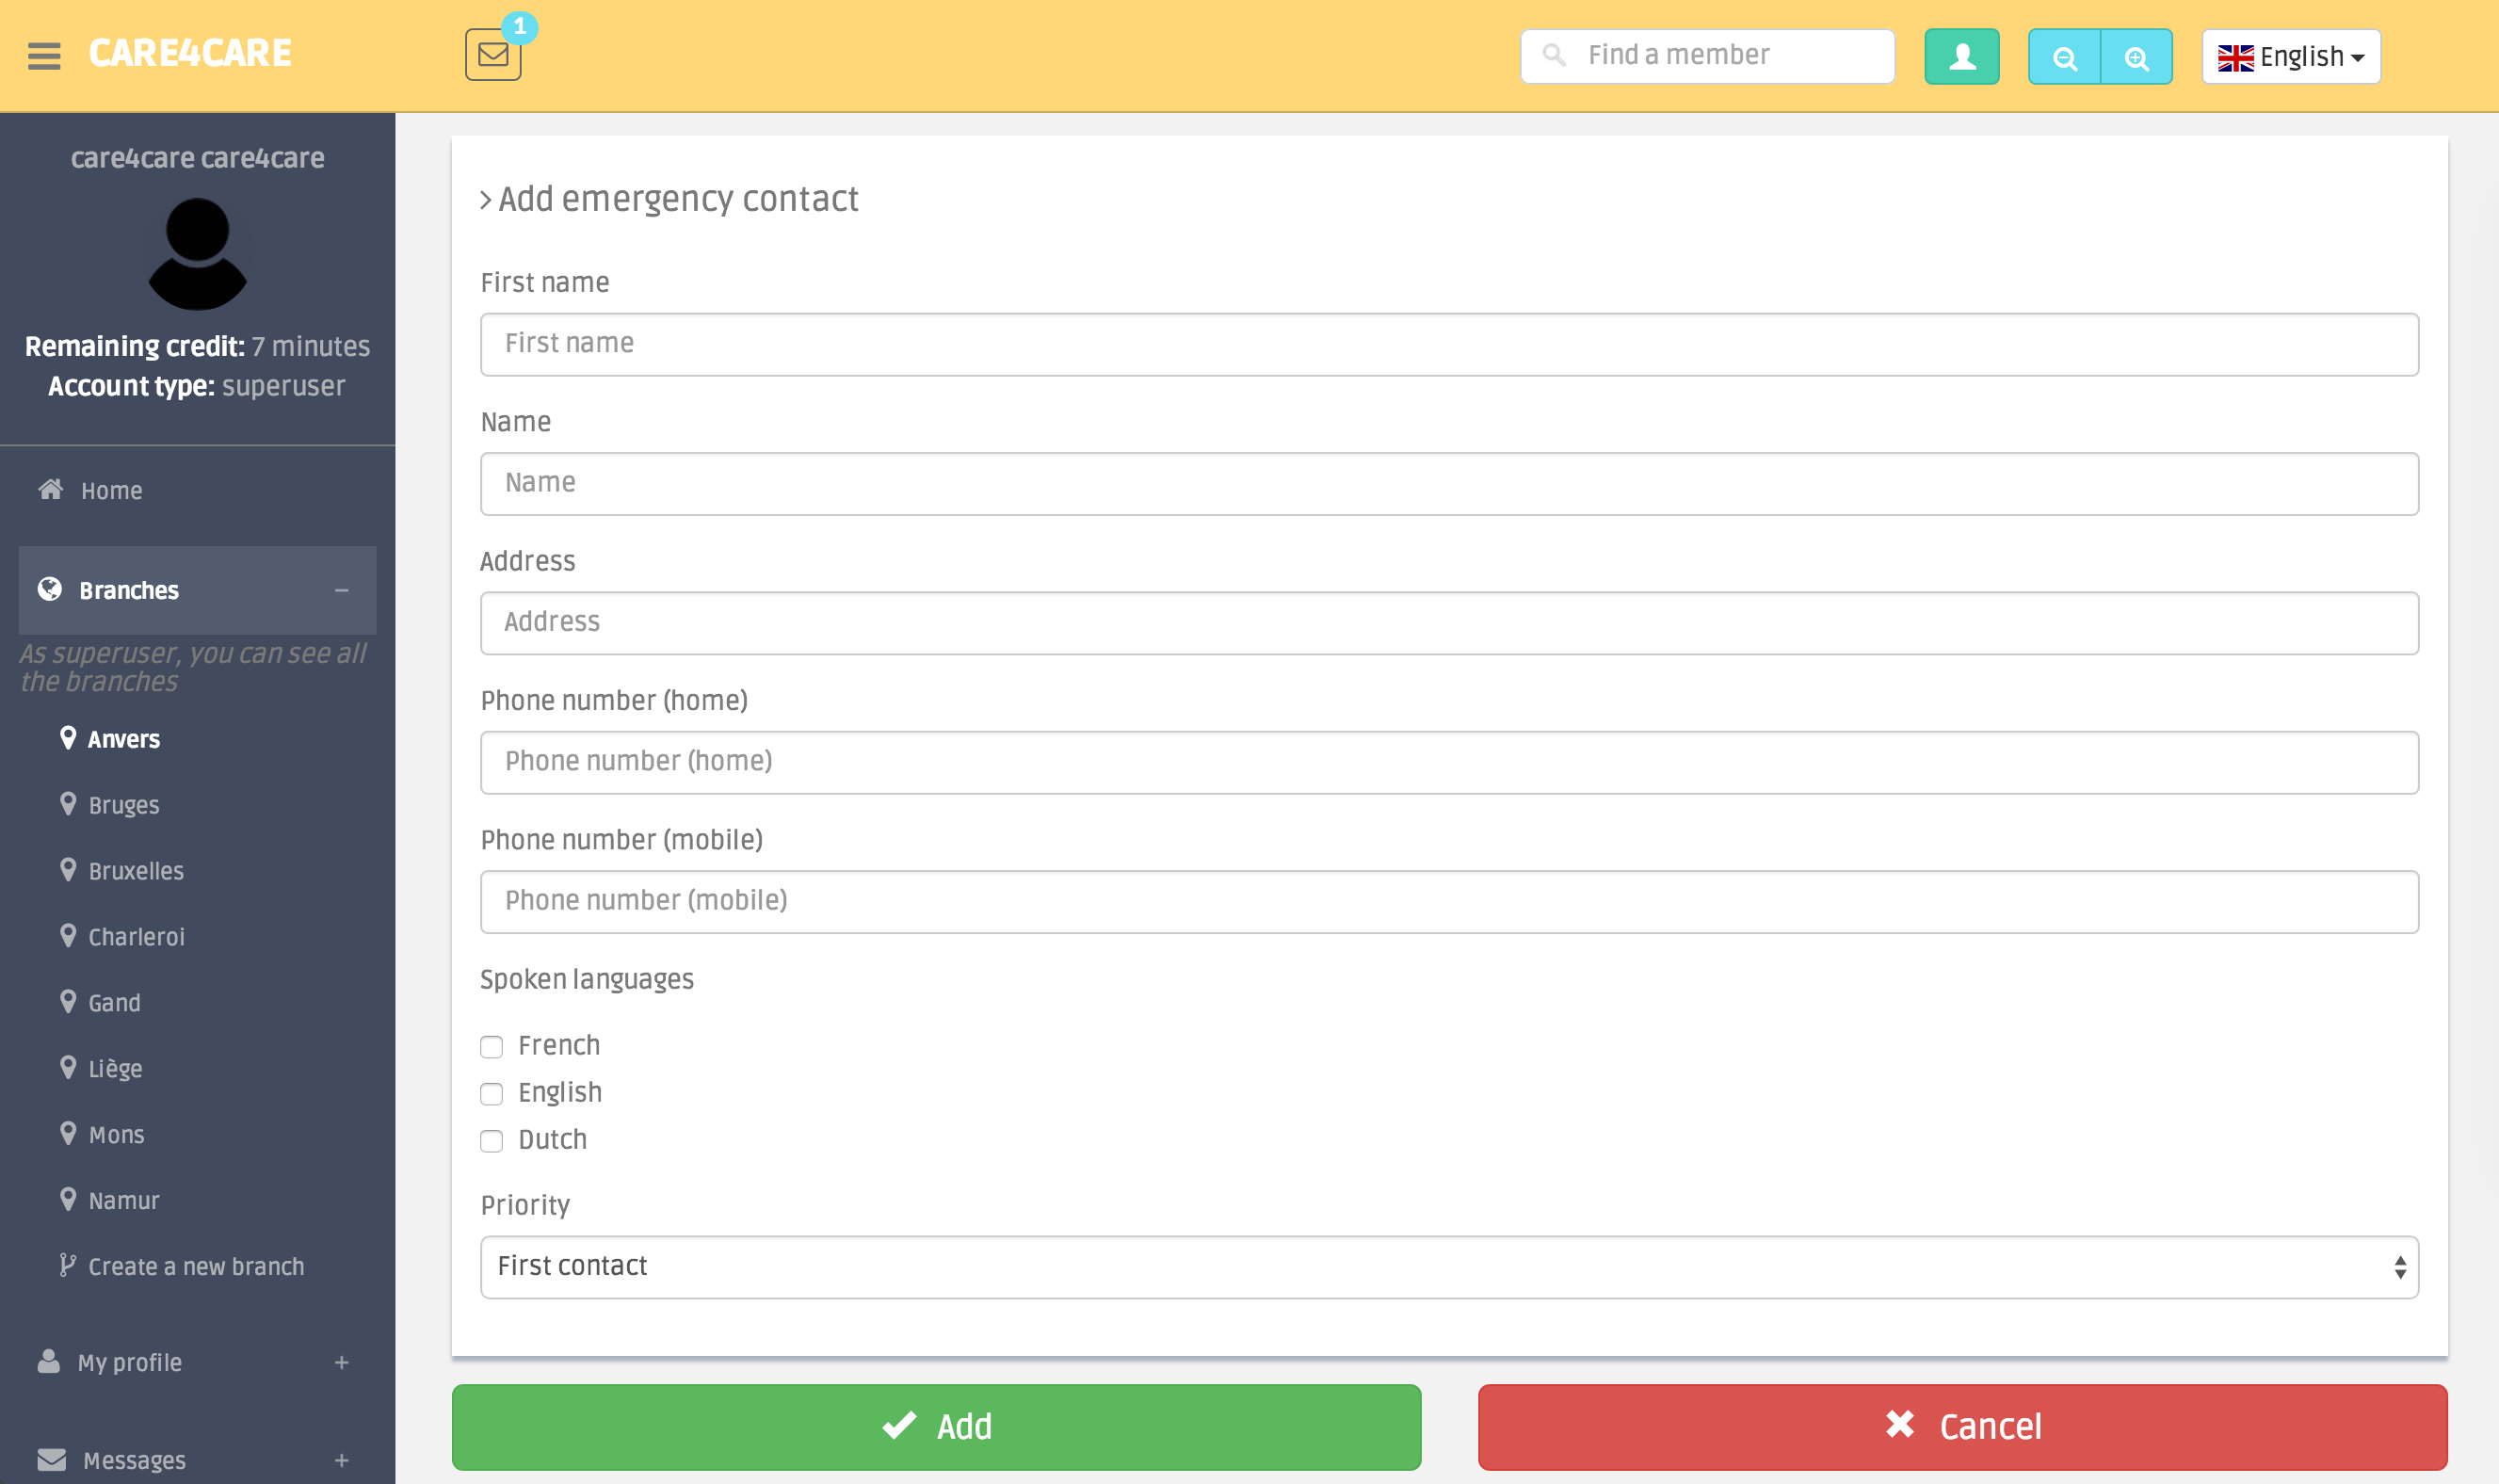
\includegraphics[width=\linewidth]{addec.png}
   \caption{Add emergency contact}
\end{figure}



\input{statistics_technical.texpart}


%%%%%% Section
\section{Translation}

Our site can be used with multiple languages. Indeed, the French and English are already fully implemented. But an additional translation can be done easily.\\
Here are some useful files for translation :

\begin{description}
\item [makelocale.sh] Generate translations
\item [compilelocale.sh] Compile translations
\end{description}
Both are used as command.\\
\\
The make generates a file \textit{django.po} that contains all the translatable elements in the code. These are defined in django through \\ \textit{from django.utils.translation import ugettext as \_}. \\
Thus, for example, \textit{\_("Veuillez choisir une adresse")} will be added to the texts to be translated in the \textit{django.po} during the make. \\
In a .html, the \textit{\% trans} to translate the message is required.\\
\\
When the make was executed, you can then translate the messages. Two choices are available to you:

Either directly edit the file django.po in locale/en/LC\_MESSAGES. The "en" folder contains the english translations and "nl" folder contains the dutch translations. For each message, there are indications of the location in the code and two fields: \textit{msgid} which contains the original message and \textit{msgstr} which contains the translation.

Either you use the Rosetta interface, accessible via the superuser by adding \textit{/translate} to the url of the site. This interface will allow you to easily change the translations. It can therefore be used by the customer.\\
\\
When the file \textit{django.po} is filled (either directly or via Rosetta), a compilation is needed to integrate these translations in the code.


%%%%%% Section
\section{Conclusion}

\end{document}
